% Chapter 1

\chapter{Theoretical framework} % Chapter title

\label{ch:thfw} % For referencing the chapter elsewhere, use \autoref{ch:name}

%----------------------------------------------------------------------------------------

\section{Deep Inelastic Scattering}

The Deep Inelastic Scattering (DIS) process is depicted in Fig.\ref{pic:DIS}. The incoming lepton $l$ exchanges
a virtual photon $\gamma^*$ with the nucleon $N$. The nucleon absorbs the energy of the virtual photon and fragments
into a final state X. The scattered lepton is represented by $l'$. This process description is also known as the
one photon exchange approximation.

% Pic DIS

The kinematics of a DIS event are fixed by the 4-momentum vector of l (\textbf{l} = ($E$,$\vec{l}$)), $l'$ (\textbf{l'} = ($E'$,$\vec{l}'$))
and N (\textbf{P} = ($M$,$\vec{0}$)). The 4-momentum vector for the virtual photon is calculated as \textbf{q} = \textbf{l} - \textbf{l'} =
($\nu$ = $E$ - $E'$, $\vec{q}=\vec{l}-\vec{l}'$). One needs only two Lorentz invariant variables to describe
inclusive DIS. One is the invariant mass of the virtual photon $Q^2$.

\begin{equation}
  Q^2 = -\textbf{q}^2 \stackrel{lab}{\approx} 4EE'sin^2(\frac{\theta}{2})
\end{equation}

$Q^2$ defines the scale at which the nucleon structure is probed : the largest $Q^2$ is, the farthest the probing
of the nucleon is performed.

The other is $x$ and measures the elasticity of the interaction. $x$ is comprised between 0 and 1. If $x=1$ the
interaction is elastic, if $x<1$ then it is inelastic. This Bjorken\cite{Bjorken} $x$ is defined as the fraction
of the nucleon 4-momentum \textbf{P} carried by the parton struck by the virtual photon.

\begin{equation}
  x = \frac{Q^2}{2\textbf{P}\cdot\textbf{q}} \stackrel{lab}{=} \frac{Q^2}{2M\nu}
\end{equation}

Other Lorentz invariant can be as well (Table\ref{tab:kinvar})

\begin{tabularx}{\textwidth}{r|lX}
  \hline
  \hline
  Variable & Description \\
  \hline
  \hline
  $Q^2 = -\textbf{q}^2 \stackrel{lab}{\approx} 4EE'sin^2(\frac{\theta}{2})$ & Interaction scale \\
  $\nu = \frac{\textbf{P}\cdot\textbf{q}}{M} \stackrel{lab}{=} E - E'$ & Energy transfer from the lepton $l$ to $\gamma^*$ \\
  $x = \frac{Q^2}{2\textbf{P}\cdot\textbf{q}} \stackrel{lab}{=} \frac{Q^2}{2M\nu}$ & \vtop{\hbox{\strut Fraction of the nucleon momentum \textbf{P} carried by the}\hbox{\strut parton struck by $\gamma^*$}} \\
  $\nu = \frac{\textbf{P}\cdot\textbf{q}}{\textbf{P}\cdot\textbf{l}} \stackrel{lab}{=} \frac{\nu}{E}$ & \vtop{\hbox{\strut Fraction of the incoming lepton energy transferred}\hbox{\strut to $\gamma^*$}} \\
  $s = (\textbf{P}+\textbf{l})^2 \stackrel{lab}{\approx} M^2 + 2ME$ & Center-of-mass energy squared \\
  $W^2 = (\textbf{P}+\textbf{q})^2 \stackrel{lab}{=} M^2 + 2M\nu - Q^2)$ & Invariant mass of the hadronic final state \\
  \hline
  \hline
\end{tabularx}

\subsection*{Cross section calculation for the inclusive DIS process}

The deep inelastic cross section, in the one photon exchange approximation, can be written in terms
of the lepton-photon coupling tensor $L_{\mu\nu}$ and the hadronic coupling tensor $W^{\mu\nu}$.

\begin{equation}
  \frac{d\sigma}{dE'd\Omega} = \frac{\alpha^2}{2Mq^4}\frac{E'}{E}L_{\mu\nu}W^{\mu\nu}
\end{equation}

$\alpha$ is the fine structure constant. The leptonic and hadronic tensors are defined by :

\begin{equation}
  L_{\mu\nu}(l,s;l') = 2{L^{(S)}_{\mu\nu}(l;l')+iL^{(A)}_{\mu\nu}(l,s;l')}
\end{equation}

where

\begin{equation}
  L^{(S)}_{\mu\nu} = l_{\mu}'l_{\nu} + l_{\nu}'l_{\mu} - g_{\mu\nu}(\vec{l}'\vec{l}-m^2) \\
  L^{(A)}_{\mu\nu} = -m\epsilon_{\mu\nu\sigma\rho}s^{\sigma}q^{\rho}
\end{equation}

and

\begin{equation}
  W^{\mu\nu}(q;P,s) = W^{\mu\nu\ (S)}(q;P) + iW^{\mu\nu\ (A)}(q;P,S)
\end{equation}

where

\begin{equation}
  \frac{1}{2M}W^{\mu\nu\ (S)}(q;P) = W_1(P\cdot q,q^2)(-g^{\mu\nu}-\frac{q^{\mu}q^{\nu}}{q^2})+\frac{W_2(P\cdot q,q^2)}{M^2}(P^{\mu}-\frac{P\cdot q}{q^2}q^{\mu})(P^{\nu}+\frac{P\cdot q}{q^2}q^{\nu})
\end{equation}

\begin{equation}
  \frac{1}{2M}W^{\mu\nu\ (A)}(q;P,S) = \epsilon_{\mu\nu\sigma\rho}q^{\sigma}{G_1(P\cdot q,q^2)MS^{\rho}+\frac{G_2(P\cdot q,q^2)}{M}(P\cdot q)S^{\rho}-(S\cdot q)P^{\rho}}
\end{equation}

The lepton and nucleon polarizations are given respectively by $s$ and $S$. $g_{\mu\nu}$ is the
Minkowski metric and m is the lepton mass. The functions $W_1(P\cdot q,q^2)$, $W_2(P\cdot q,q^2)$,
$G_1(P\cdot q,q^2)$ and $G_2(P\cdot q,q^2)$ are the spin averaged and spin dependent structure functions
parametrizing the internal structure of the nucleon. They can be expressed as dimensionless functions as
in Eqs.\ref{} to \ref{}.

\begin{equation}
  MW_1(P\cdot q,Q^2)=F_1(x,Q^2)
  \nu W_2(P\cdot q,Q^2)=F_2(x,Q^2)
  \frac{(P\cdot q)^2}{\nu}G_1(P\cdot q,Q^2)=g_1(x,Q^2)
  \nu(P\cdot q)G_2(P\cdot q,Q^2)=g_2(x,Q^2)
\end{equation}

Going back to Eq.\ref{} and splitting the symmetric and antisymmetric parts of the tensors :

\begin{equation}
  \frac{d\sigma}{dE'd\Omega} = \frac{\alpha^2}{2Mq^4}\frac{E'}{E}[L_{\mu\nu\ (S)}W^{\mu\nu\ (S)}-L_{\mu\nu\ (A)}W^{\mu\nu\ (A)}]
\end{equation}

After summing over all possible spin configurations of the initial and final lepton and nucleon, neglecting
the leptonic mass, one obtains the unpolarized DIS cross-section (Eq.\ref{}) which measurement gives access
to the structure functions $F_1$ and $F_2$.

\begin{equation}
  \frac{d\sigma^{unpolarized}}{dxdQ^2} = \frac{4\pi\alpha}{Q^4}[y^2F_1(x,Q^2)+(\frac{1-y}{x}-\frac{My}{2E})F_2(x,Q^2)]
\end{equation}

%------------------------------------------------

\section{Quark Parton Model}

The Quark Parton Model is developed in the infinite momentum frame where the nucleon has a very large momentum
along a certain direction and is composed by massless point-like particles called partons. In this case, the
transverse momentum of these partons can be neglected. In DIS, the virtual photon interacts with the parton,
which carries a fraction $\xi$ of the 4-momentum \textbf{P} of the nucleon and the invariant mass of the initial
and final states are respectively $(\xi\textbf{P}+\textbf{q})^2$ and 0. This yelds :

\begin{equation}
  (\xi\textbf{P}+\textbf{q})^2 = 0 \Rightarrow 2\xi\textbf{P}\cdot\textbf{q}+\textbf{q}^2 = 0 \Rightarrow \xi = \frac{Q^2}{2\textbf{P}\cdot\textbf{q}}
\end{equation}

which is the exact definition of Bjorken $x$.

Within this model, since gluons do not carry any electric charge, the DIS interaction can only involve quarks and
it has to be noted that the surrounding quarks are not affected by the interaction. The hadronic tensor is defined
by Eq.\ref{}.

\begin{equation}
  W^{\mu\nu} = \sum\limits_{q,s}e^2_qn_q(x,s;S)\frac{1}{\textbf{P}\cdot\textbf{q}}[2x\textbf{P}^{\mu}\textbf{P}^{\nu}
  +\textbf{P}^{\nu}\textbf{q}^{\mu}+\textbf{P}^{\mu}\textbf{q}^{\nu}-g^{\mu\nu}\textbf{P}\cdot\textbf{q}]
\end{equation}

where $n_q(x,s;S)$ is the density of quarks q with charge $e_q$ and spin $s$, the nucleon spin being given by S.
In this model, the structure functions expressions are :

\begin{equation}
  F_1(x)=\frac{1}{2}\sum\limits_{q}e^2_qq(x) \\
  F_2(x)=x\sum\limits_{q}e^2_qq(x)
\end{equation}

where $q(x)$ are the unpolarized Parton Distribution Functions (PDFs). The sums run over all quark flavors.
One can draw a trivial relationship between $F_1$ and $F_2$, called the Callan-Gross relation :

\begin{equation}
  F_1(x)=\frac{1}{2x}F_2(x)
\end{equation}

As the QPM is considered inside the infinite momentum frame, $Q^2 \rightarrow \infty$ and the $Q^2$ dependence of
$F_1$ and $F_2$ is thus lost : this sclaing violation is also known as the Bjorken scaling. This observation along
with the Callan-Gross relation showed that partons are indeed 1/2-spin particles.

Eventually yields the unpolarized DIS cross-section with the QPM :

\begin{equation}
  \frac{d^2\sigma^{unpolarized}}{dxdy} \stackrel{QPM}{=} \frac{8\pi\alpha^2ME}{Q^2}[\frac{1}{2}y^2+(1-y-\frac{y^2\gamma^2}{4})]x\sum\limits_{q}e^2_qq(x)
\end{equation}

\subsection*{Scaling violation}

The structure function $F_2$ has been measured by several collaborations covering a wide $x$ - $Q^2$ kinematic range.
The measured values are plotted as a function of $Q^2$ and in bins of $x$. The Bjorken scaling is only visible in a
small $x$ region between 0.1 and 0.4. Outside this region the structure function $F_2$ has a logarithmic dependence on
$Q^2$. At small $x$, $F_2$ increases with $Q^2$ while at large $x$, $F_2$ decreases for large $Q^2$ values. From the scaling
violation a conclusion was made that there should be a missing piece in the QPM : the gluon contribution. In order to take
into account this contribution, the QPM was developed within the Quantum ChromoDynamics frame (QCD).

%Pic F2 scaling violation

\subsection*{QCD-improved QPM}

The $Q^2$ dependence observed in previous subsection can be estimated by introducing the quark interaction from QCD.
Quantum ChromoDynamics is a non-abelian gauge theory based on a symmetry group SU(3) which describes the strong interaction.
The charge of this theory is called colour and the force carriers are the gluons, which are also coloured particles. The
internal nucleon dynamic is dominated by the gluon emission and absorption by the 3 valence quarks. The gluons can create
pairs of quark-antiquark or emit gluons. This creates a cloud of gluons and virtual $q\bar{q}$ pairs known as sea quarks.

The QCD coupling constant $\alpha_s$ depends on the scale of the interaction. At low energies quarks or gluons are always
forming colorless particles as hadrons : this is the confinement. At high energies quarks or gluons are free particles :
this is asymptotic freedom.

Depending on the energy regime, a process can be labeled as a hard ($\alpha \sim 0$) or soft process ($\alpha \approx 0$).
Hard processes can be described within the perturbative QCD (pQCD) framework when soft processes can only be parametrized
from experimental data. This two regimes differ by the factorisation scale $\Lambda$. As in DIS the scale variable is $Q^2$,
the DIS cross-section can only be factorized in terms of soft and hard processes at $Q^2>1$GeV$^2$ : the hard process is the
lepton-quark interaction $\sigma_q$ and the soft process is a non-calculable universal quantity which are the PDFs.

The resolution of the virtual photon probe is proportional to $1/Q^2$ (Fig.\ref{}). At $Q^2 \approx 0$, the virtual photon sees the
nucleon as a point-like particle. As $Q^2$ increases, the virtual starts to interact with the nucleons constituents. At large $Q^2$
the virtual photon is able to access the gluons. The first QCD correction to the QPM concerns the gluon emission by the initial and
the final quark. The splitting functions $P_{ij}(x/\xi)$ are the probability that a quark or gluon of type $j$ and momentum fraction
$\xi$ is the parent of i with momentum fraction $x$.

% pic res photon

The $Q^2$ dependence is calculated by the Dokshiter-Gribov-Lipatov-Altarelli-Parisi (DGLAP) equations.

\begin{equation}
  \frac{dq_i(x,Q^2)}{dlnQ^2} = \frac{\alpha_s(Q^2)}{2\pi}\sum\limits_{j}\int_{x}^{1}P_{ij}(x/\xi,\alpha_s(Q^2))q_i(\xi,Q^2)
\end{equation}

If the PDFs are known at a given scale $Q_0^2$, they can be evolved to any given $Q^2$ using these equations.

%----------------------------------------------------------------------------------------

\section{Determination of Parton Distribution Functions}

The PDFs are non-perturbative quantities and thus cannot be devised from a theoretical framework. A global fit to world data is the
only way to quantify them. This global fit is only possible because PDFs are universal quantities, ie. they are process independent.
The world data consists of lepton-nucleon DIS, collider experiments ($pp$ or $p\bar{p}$), neutrino scattering, etc. As experiments
cover different kinematic ranges, this allow one to determine the PDFs in a large ($x$,$Q^2$) space.

For the fit to be performed, a functional form has to be provided at $Q^2_0$. They are usually following the form : $xq_i(x,Q^2_0) = x^{\alpha}(1-x)^{\beta}$
with following terms refining the fit, reaching a number of free parameters from 10 to 25. The DGLAP equations are then used to evolve
the PDFs to a given $Q^2$. An example of a fit done by the MMHT group at Next to Leading Order (NLO) for different $Q^2$ values is shown in Fig.\ref{fig:MMHT}.

\begin{figure}[htb!]
\centerline{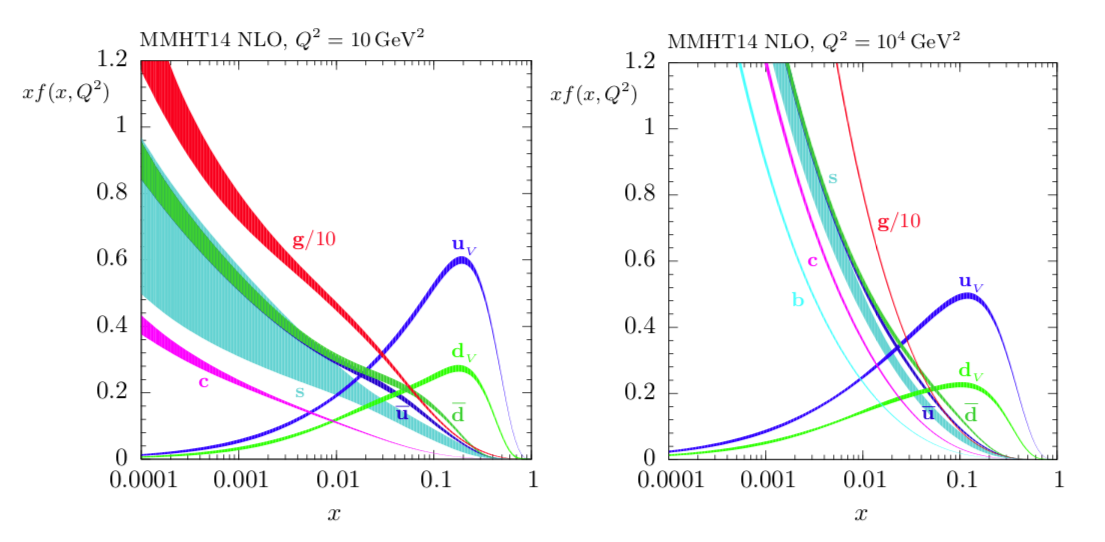
\epsfig{file=gfx/MMHT.png,width=14cm}}
\caption{Unpolarized PDFs at Next to Leading Order (NLO) from MMHT group at $Q^2$ = 10 GeV$^2$ (left) and $Q^2$ = 10$^4$ GeV$^2$ (right) with associated 68\%
confidence-level uncertainty bands. Figure taken from \cite{MMHT}.}\label{fig:MMHT}
\end{figure}

%----------------------------------------------------------------------------------------

\section{Semi-Inclusive Deep Inelastic Scattering}

As its name induces, Semi-Inclusive Deep Inelastic Scattering (SIDIS) is the semi-inclusive channel of the overall DIS process. In the
final state, a hadron and the scattered lepton are detected ($l+N \rightarrow l'+h+X$) and a new invariant variable $z$ is introduced,
which corresponds to the energy fraction of the virtual photon held by the hadron $h$ (Eq.\ref{}).

\begin{equation}
  z = \frac{\textbf{P}\cdot\textbf{p}_h}{\textbf{P}\cdot\textbf{q}} \stackrel{lab}{=} \frac{E_h}{\nu}
\end{equation}

The semi-inclusive cross section reads \cite{}:

\begin{equation}
  \frac{d\sigma}{dxdydz} \stackrel{QPM}{=} \frac{8\pi\alpha^2ME}{Q^4}[xy^2H_1(x,Q^2,z)+(1-y)H_2(x,Q^2,z)]
\end{equation}

where $H_1$ and $H_2$ are structure functions related to $F_1$ and $F_2$ \cite{} :

\begin{equation}
  \sum\limits_{h}\int_{0}^{1} H_i(x,Q^2,z)dz = F_i(x,Q^2), i \in  \llbracket1,2\rrbracket
\end{equation}

Other variables can be used to describe the hadron in SIDIS (Table.\ref{}).

\begin{tabularx}{\textwidth}{r|lX}
  \hline
  \hline
  Variable & Description \\
  \hline
  \hline
  $\textbf{p}=(E_h,\vec{p}_h)$ & Hadron 4-momentum vector \\
  $p_{h\|}$ & Component of $\vec{p}_h$ along $\vec{q}$ \\
  $p_{h\bot}$ & Transverse component of $\vec{p}_h$ with respect to $\vec{q}$ \\
  $\theta_h$ & Angle between $\vec{q}$ and $\vec{p}_h$ \\
  $\Phi_h$ & Angle between the scattering plane and the hadron production plane \\
  $z$ & Energy fraction of the virtual photon transferred to the hadron $h$ \\
  \hline
  \hline
\end{tabularx}

\subsection*{SIDIS in QPM}

The factorization theorem allows to describe the hadron production as two independent processes : the hard process $\sigma_q$
describing the absorption of the virtual photon $\gamma^*$ by the quark $q$ and the soft process $D_q^h(z)$ ruling the
fragmentation of the quark $q$ into a hadron $h$.

% pic sidis feynman

The structure functions $H_i(x,Q^2,z)$ contain the information on what happens to the struck quark after the interaction with
the virtual photon. The fragmentation function (FF) $D_q^h(z,Q^2)$ is defined as the probability for a quark of flavour $q$ to fragment
into a hadron $h$ with a fraction of energy $z$. The expression of the SIDIS cross section can be expressed at LO in terms of the PDFs and
the FFs \cite{} :

\begin{equation}
  \frac{d^3 \sigma^{unpolarized}}{dxdydz} \stackrel{LO}{=} \frac{8\pi\alpha^2ME}{Q^2}[\frac{1}{2}y^2+(1-y-\frac{y^2 \gamma^2}{4})]x\sum\limits_qe^2_qq(x)D_q^h(z)
\end{equation}

\subsection*{Scaling and $Q^2$ evolution}

A scaling violation is observed for the FFs extracted from $e^+e^-$ annihilation \cite{}. The scaling is present in the $x = 2p_h/\sqrt{s}$
bin 0.1-0.2. At low x ($x$ < 0.1) the FFs increases with $\sqrt{s}$, while at large $x$, the FFs are shifted towards lower values for large
$Q^2$.

% pic scaling violation

The evolution of the fragmentation functions is done with the DGLAP equations \cite{} :

\begin{equation}
  \frac{dD_q^h(z,Q^2)}{dlnQ^2} = \frac{\alpha_s(Q^2)}{2\pi}\sum\limits_j\int_{x}^{1}P_{qj}(z/\xi,\alpha_s(Q^2))D_q^h(\xi,Q^2)\frac{d\xi}{\xi}
\end{equation}

In Fig.\ref{} is shown the fragmentation of quark and gluons. Four different fragmentation channel can be separated : the fragmentation of a quark
$q_i$ through its own decay after emmiting a gluon G ($P_{qq}D_{q_i}^h$), through the decay of a gluon G ($P_{Gq}D_{G}^h$), the fragmentation of a
gluon splitting into a quark-antiquark pair and following hadronization of the quark in hadron ($P_{qG}D_{q_i}^h$) and eventually the gluon
fragmentation via the three-gluon self-interaction ($P_{GG}D_{G}^h$).

%----------------------------------------------------------------------------------------

\section{Fragmentation Functions}

The FFs describes the hadronization ie. the quark fragmentation into a hadron. The quark fragmentation into a hadron is a soft process and cannot
be described using pQCD. Different models have been developed to describe how quarks confine together to make a hadron.

\subsection*{Lund String Fragmentation Model}

In the Lund String Model \cite{}, the hadron production is explained by the creation of quark-antiquark pairs $q\bar{q}$. The strong interaction between
partons is represented by a string. The energy inside the string is linear function of the distance between two stringed partons. At some point the
energy is large enough to create a new $q\bar{q}$ pair and the string breaks. Each paired remnants have new strings and the process repeats until there
are only hadrons. The hadronization scheme in the Lund model in the center of mass frame is illustrated in Fig.\ref{}. The virtual photon is absorbed by
the $u$ quark and in consequence the $u$ quark is ejected from the nucleon. The remaining $u$ quark bounds with the $\bar{d}$ quark to form a $\pi^+$
with a given $z$ (see Table\ref{}). The remaining system repeats fragmentation process until the energy is smaller than the available energy $\nu$.

\subsection*{Quark Fragmentation Regions}

At this point only the production from struck quarks were considered. Nevertheless, it is also possible that a spectator quark which is not involved in
the scattering process fragments into hadrons. This phenomenon is happening in two well $p_h$-defined regions : the target fragmentation region where
the final hadron $h$ has a small momentum in the rest frame of the target and the current fragmentation region where the product $\textbf{P}\cdot\textbf{p}_h$
grows with $Q^2$. This hadron production can contaminate the hadron production from the actual SIDIS process. To deal with this issue, Berger \cite{} came
with a criterion based on the rapidity of the final state $\eta$. The sign of $\eta$ is linked to the different regions : if $\eta$ > 0 the hadron moves
towards the direction of the virtual photon and is a current hadron, else is $\eta$ < 0 the hadron is a target remnant (Fig.\ref{}). As the typical hadronic
correlation length in rapidity is $\delta \sim 2$, a separation criterion, the Berger criterion, is that $\Delta\eta = \eta_{max}-\eta_{min} \geq 2\delta$
or in terms of DIS kinematics variables $W \gtrsim 7.4$ GeV. It is important to be able to separate the current and target fragmentation to ensure the quark
fragmentation into hadrons is independent of the production of the quark.

%----------------------------------------------------------------------------------------

\section{Measurement of Fragmentation Functions}
